\chapter{Metodologia Científica}

\begin{center}
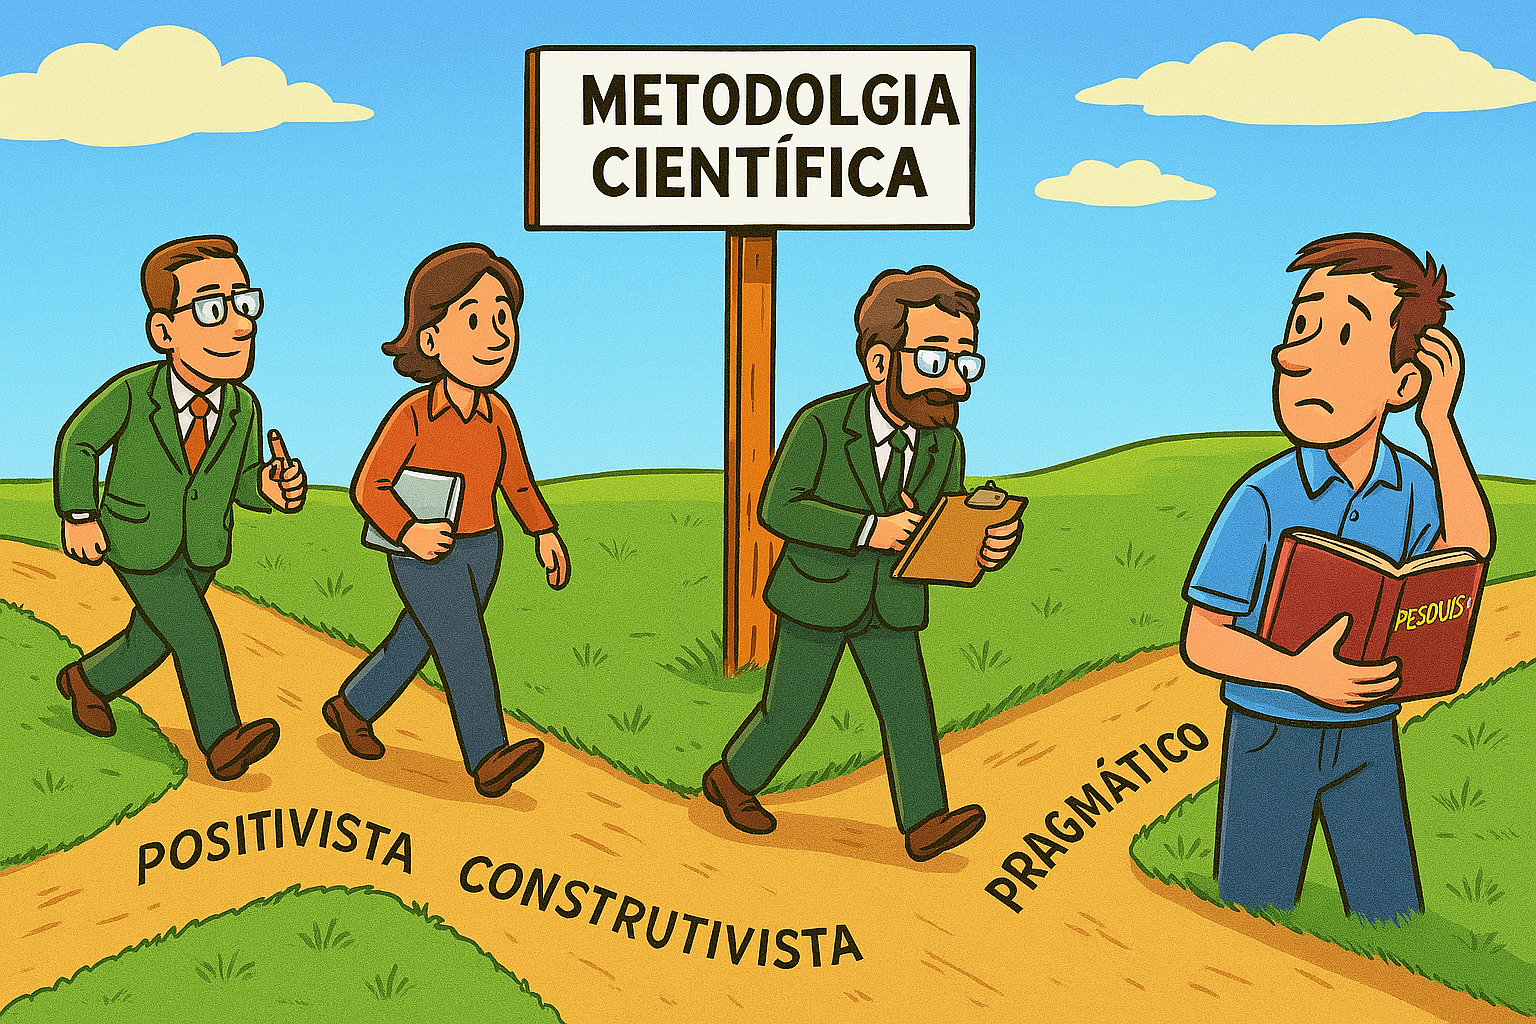
\includegraphics[width=0.5\linewidth]{Images/metodologia.png}    
\end{center}
\vspace{0.5cm}



Não pretendemos, neste capítulo, fazer uma discussão complexa do que é o método científico, mas mostrar algumas noções básicas que devem ser pensadas \textbf{antes} ao começar o trabalho. 

A escolha explícita e consciente do método científico frente a um contexto e questão de pesquisa é complexa e depende de vários fatores. 
Porém, na prática, ela acaba sendo muitas vezes implícita, pois é feita na base da cópia, adaptação e evolução das práticas usadas pelo grupo com que trabalha, que têm grande impacto nessa escolha. 

Uma pesquisa se baseia em uma perspectiva filosófica, ou paradigma filosófico, que muitas vezes é implícita. 
Existem várias perspectivas filosóficas, e \citet{creswell2021projeto} chamam a atenção para quatro: a positivista e pós-positivista, a construtivista, a transformativa e a pragmática. 

Esses quatro paradigmas diferem fundamentalmente em suas concepções de realidade, conhecimento e o papel do pesquisador. O \gxdefine{paradigma positivista} e pós-positivista busca a objetividade, baseando-se em métodos quantitativos para testar hipóteses e estabelecer leis gerais por meio de mensuração e experimentação. Já o \gxdefine{paradigma construtivista} enfatiza a construção social da realidade, valorizando a subjetividade e a interpretação, com forte predileção por métodos qualitativos, como entrevistas e observações. \gxdefine{O paradigma transformativo}, por sua vez, está comprometido com a justiça social e a emancipação de grupos marginalizados; ele frequentemente adota métodos mistos, combinando abordagens quantitativas e qualitativas para dar voz a participantes e provocar mudanças estruturais. Por fim, o paradigma pragmático é orientado pela resolução de problemas e pela utilidade prática do conhecimento, e por isso tende a adotar métodos mistos de forma flexível, escolhendo técnicas com base em sua eficácia para responder às questões de pesquisa~\citet{creswell2021projeto}.

Não cabe a este texto entrar profundamente no tema, mas é possível que seu  grupo de trabalho, mesmo não ``sabendo'', esteja envolvido com um paradigma específico. 
Por exemplo, é comum que pesquisas em Engenharia sigam a perspectiva positivista ou pós-positivista, enquanto as áreas de Humanas têm escolhido muitas vezes o paradigma transformativo.
Principalmente o candidato ao doutorado tem muito a ganhar entendendo qual o paradigma de pesquisa que segue, ou que deveria estar seguindo, e quais métodos e atividades de pesquisa são mais adequados no contexto.

Fica aqui, porém, um aviso: é difícil defender uma tese dentro de um ambiente que adota um paradigma filosófico usando outro paradigma. 

\section{O Método Científico}

Partimos de uma visão do método científico que é bastante geral, apresentada por \citet{Bunge2002}, que é uma visão epistemológica da investigação científica como uma sequência de atividades~\citep[p. 39-40]{Bunge2002}\footnote{Tradução livre do autor}:
\begin{quote}
\begin{enumerate}
    \item Descobrimento do Problema ou lacuna em um conjunto de conhecimentos. Se o problema não está enunciado com clareza, se passa à etapa seguinte, se não, à subsequente;
    \item Descrição precisa do problema, se possível em termos matemáticos, mas não necessariamente quantitativos, ou uma nova descrição de um velho problema a luz de novos conhecimentos 
    \item Busca de conhecimentos ou instrumentos relevantes ao problema (por exemplo, dados empíricos, teorias, aparatos de medida, técnica de cálculo ou de medida). Ou seja, inspeção do conhecido para ver se é possível resolver o problema;
    \item Tentativa de solução do problema com ajuda dos meios identificados. Se essa tentativa falha, passasse à etapa seguinte, se não, à subsequente.
    \item Invenção de novas ideias (hipóteses, teorias ou técnicas) ou a produção de novos dados empíricos que prometam resolver o problema;
    \item Obtenção uma solução, exata ou aproximada, do problema com auxílio do instrumental conceitual ou material disponível;
    \item Por a prova a solução, por exemplo, com ensaios de laboratório ou de campo, e
    \item Correções necessárias nas hipóteses ou técnicas, ou mesmo na formulação do problema original.
\end{enumerate}
\end{quote}

Essa descrição, ilustrada na Figura \ref{fig:bunge}, é o que se chama na Engenharia de Software de um processo Linear ou em Cascata, mas é óbvio que isso é só uma abstração que facilita a descrição a nível epistemológico. A pesquisa científica é um processo de aprendizado constante, e muitas vezes é necessário, após uma etapa, voltar atrás, ou pular à frente, de forma a melhorar a compreensão do problema, das soluções possíveis, corrigir experimentos, etc.

\begin{figure}[hbt]
    \centering
	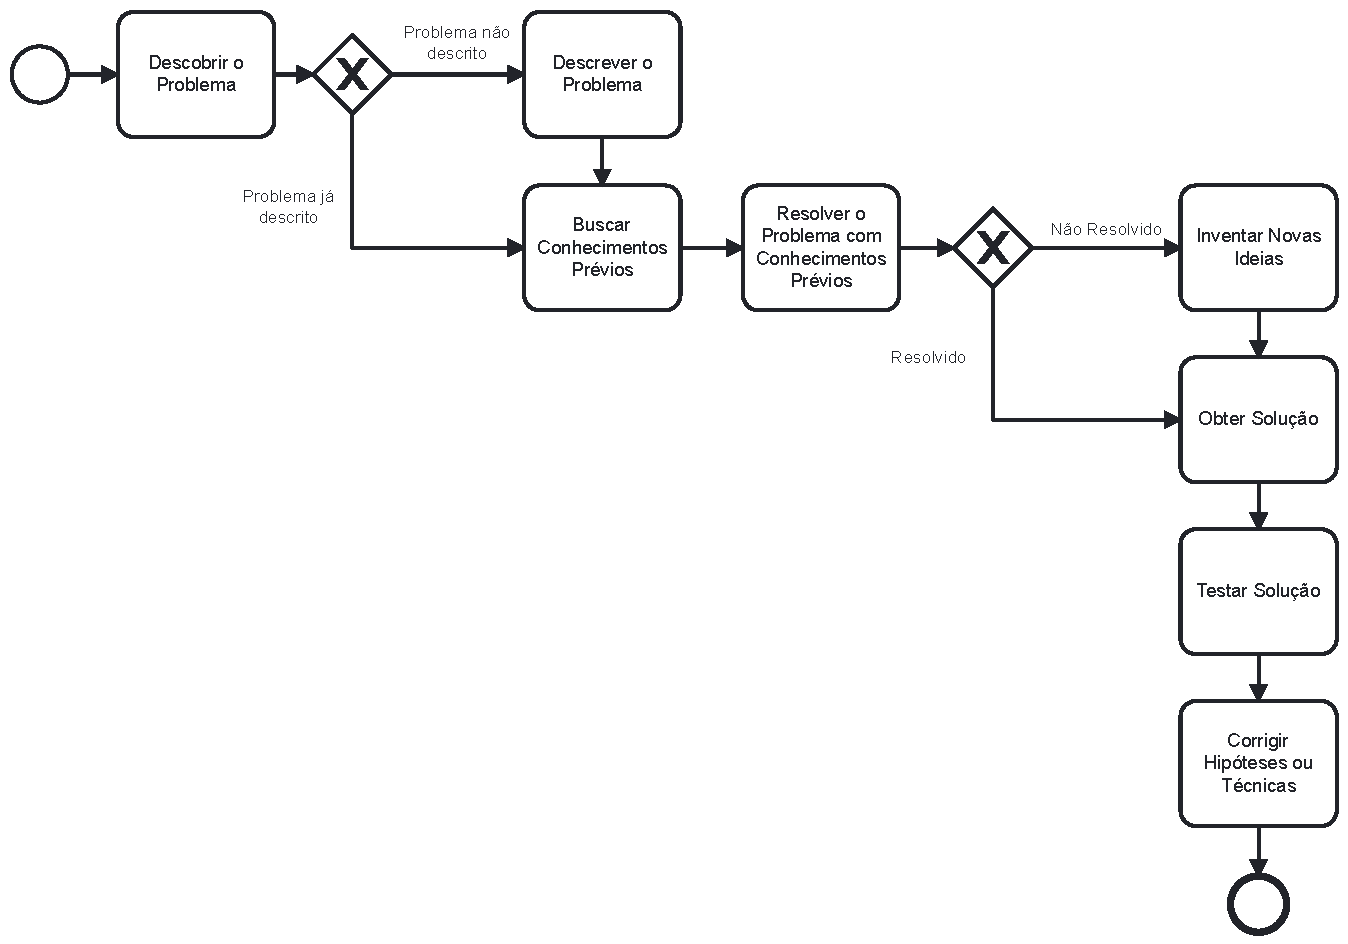
\includegraphics[width=0.7\linewidth]{Images/metodologiabunge.pdf}
    \caption{Metodologia Científica segundo \citet{Bunge2002}, descrita em BPMN~\citep{omg2013bpmn}. Fonte: Do Autor}
    \label{fig:bunge}
\end{figure}

O Mario Bunge ainda diz que para que uma ideia seja considerada científica é necessário, mas não suficiente, que ela seja objetivamente testável com dados empíricos~\citep[p. 37]{Bunge2002}\footnote{Essa sentença segue um dos princípios centrais do realismo científico sistemático e do pós-positivismo crítico caracterizado por Bunge.}.

Ainda mais, \citet[p. 40]{Bunge2002} cita \citet{Kuhn1970}, que diz que a melhor forma de aprender a planejar e resolver problemas científicos não é estudar um manual de metodologia, mas \textbf{estudar e imitar paradigmas ou modelos de investigações que tiveram êxito}. \citet{Kuhn2018}, em seu posfácio de 1969, cita outro autor, Michael Polanyi,  e defende o conhecimento tácito,  dizendo que ele ``é aprendido fazendo ciência, ao invés de adquirindo regras para fazê-la''~\citep[p. 160]{Kuhn2018}\footnote{O que é um sinal de aviso sobre este texto!}. 

Analisando estas falas, podemos concluir que mais do que decorar métodos e segui-los rigidamente, o importante é praticar a ciência e se aproveitar das lições aprendidas.

Escolhendo um método científico muito específico, por exemplo, uma variante da\textit{ Design Science Research}\citep{hevner2004design,Pimentel2019}, o candidato deve estar ciente das questões envolvidas, e ao seguir ou adaptar método, compreender o motivo de suas decisões. 

Essa questão precisa ser discutida, e tratada entre orientador e orientado.

\section{Propor e Comprovar}

Uma tese é uma proposta científica que avança o estado da arte. 
Ou seja, ao escrever sua tese você está se propondo a melhorar alguma coisa. 
Mas não basta apenas a sua opinião de que algo realmente melhorou, ou seja, que sua contribuição é útil: é necessário comprovar essa melhora.

Na abordagem empírica, é necessário construir um experimento ou fazer uma observação. Em uma abordagem teórica, as necessidades podem incluir provar um teorema.

Basicamente existem duas formas de comprovar algo: quantitativamente ou qualitativamente. No primeiro caso, você terá números claros que indicam a melhoria. Por exemplo, após rodar várias vezes dois algoritmos, em diferentes bases de dados, você pode concluir que um é duas vezes mais rápido do que o outro. Já ao comparar duas interfaces em um sistema, você pode fazer perguntas em aberto e fazer, qualitativamente, comparação subjetiva.


Lembre-se do que falou Werner Von Braun:
\gxatencao{Um resultado de um teste vale um milhão de opiniões de especialistas.}

Experimentos se tornam cada vez mais essenciais como forma de comprovação nas teses de STEM e que propõem artefatos. Se no passado a própria proposta era considerada uma contribuição, ou se em alguns lugares isso ainda é aceito, principalmente para níveis de TCC e mestrado, a tendência atual é que um aluno não vá defender um trabalho científico sem algum tipo de tentativa de comprovação científica de sua proposta, mesmo que seja limitada a um contexto específico.

Nesse ponto, é importante lembrar que propostas de artefatos, como softwares dedicados a melhorar algum desempenho humano, dificilmente podem ser comprovadas como melhorias absolutas em todos os casos, já que seus testes são feitos com grupos limitados de pessoas, dentro de contextos específicos. Mesmo sistemas testados com grandes bases de dados estão limitados, em suas conclusões, aos dados usados.

% Não confie cegamente na Internet.  Utilize o senso crítico e analise a importância da referência que está usando. Revistas indexadas são importantes fontes, congressos também. Outra fonte boa de artigos, principalmente para se aprofundar em um tema, são os relatórios técnicos produzidos pelas universidades. 

\section{Termos Importantes}
\begin{itemize}

    \item \textbf{Empírico}: Termo usado para designar conhecimentos ou abordagens baseados em observação direta, experimentação ou análise de dados reais. Na pesquisa científica, métodos empíricos são fundamentais para validar hipóteses, avaliar fenômenos e sustentar conclusões com evidências concretas.

  \item \textbf{Premissa}: Proposição aceita como verdadeira ou ponto de partida lógico sobre o qual se baseia um argumento ou raciocínio. Exemplo: ``Algoritmos de aprendizado de máquina podem ser aplicados à detecção de doenças cardíacas.''

  \item \textbf{Hipótese}: Suposição fundamentada que se pretende testar empiricamente. É uma afirmação passível de verificação que busca explicar um fenômeno ou prever um resultado. Exemplo: ``A aplicação da Transformada Wavelet melhora a acurácia da detecção de arritmias.''

  \item \textbf{Hipótese Nula} (\textit{H\textsubscript{0}}): Formulação contrária à hipótese de pesquisa, utilizada como ponto de comparação estatística. Assume que não há efeito, relação ou diferença significativa. Exemplo: ``A Transformada Wavelet não tem impacto significativo na acurácia da detecção de arritmias.''

  \item \textbf{Tese}: Afirmação central que será defendida ou demonstrada ao longo do trabalho. Pode sintetizar a conclusão antecipada da pesquisa. A tese é uma proposição central que o pesquisador defende ao longo do trabalho. Ela expressa a ideia principal ou conclusão que será sustentada com base em argumentos, dados e evidências. Pode ser resultado da validação de uma hipótese, mas também pode emergir de interpretações teóricas ou reflexões críticas. A tese representa o posicionamento do autor após o processo investigativo.

  \item \textbf{Objetivo}: Intenção geral que orienta a pesquisa; representa o que se busca alcançar de forma ampla. Exemplo: ``Propor uma estratégia eficiente para a classificação de arritmias em sinais de ECG.''

  \item \textbf{Objetivo Específico}: É um desdobramento operacional do objetivo geral da pesquisa. Define, de forma clara, concreta e mensurável, as etapas intermediárias que devem ser alcançadas ao longo do trabalho. Cada objetivo específico deve contribuir diretamente para o cumprimento do objetivo geral, orientando atividades como levantamento bibliográfico, desenvolvimento de métodos, experimentação e análise dos resultados. Eles devem ser redigidos com verbos no infinitivo (como ``analisar'', ``comparar'', ``desenvolver'', ``avaliar'') e evitar ambiguidade ou formulações excessivamente amplas.

  \item \textbf{Meta}: Resultado específico, mensurável e atingível dentro de um prazo determinado. Geralmente associada ao planejamento e execução do projeto. Exemplo: ``Treinar um modelo com acurácia superior a 90\% em um conjunto de validação.''

  \item \textbf{Questão de Pesquisa}: Pergunta central que guia a investigação e delimita o escopo do estudo. Exemplo: ``É possível classificar arritmias em sinais de ECG com alta precisão usando apenas recursos computacionais locais?''
\end{itemize}


\section{Caminhos Que Podemos Tomar}



% Não quero fazer aqui uma grande descrição desses paradigmas, mas a pós-positivista é a mais tradicional e muito ligada às abordagens quantitativas, enquanto a construtivista é mais ligada às qualitativas. 
% A transformativa tem relação com perspectivas sobre os grupos tradicionalmente marginalizados. Finalmente, a pragmática, ligada a métodos mistos e que surge de ações e consequências mais do que condições anteriores. 

O trabalho científico pode ser classificado segundo diferentes critérios, dependendo da natureza do problema, dos objetivos do estudo, do tipo de dado coletado, do papel do pesquisador, etc. 
Embora não exista uma única taxonomia universal aceita, a literatura de metodologia, apresenta algumas divisões amplamente utilizadas. 
A seguir, mostro escolhas que podem ser feitas ao fazer sua tese, e como são denominadas. 
Elas são melhor discutidas em outros livros, mas esta introdução pode ajudá-lo a pensar.

%\subsection{Teórico vs. aplicado}

% A primeira distinção relevante é entre pesquisa teórica e aplicada.

% A pesquisa teórica concentra‑se na formulação, abstração e análise de conceitos, modelos e algoritmos.  
% Busca gerar conhecimento fundamental, caracterizado por provas formais, generalidade e rigor lógico.  
% Resultados típicos incluem teoremas, \textit{frameworks} conceituais ou modelos preditivos cuja validade independe de aplicações imediatas.

% A pesquisa aplicada é direcionada à resolução de problemas práticos com base em teorias existentes ou artefatos novos. 
% Ela é predominante nas dissertações de mestrado profissional e trabalhos de Engenharia.

% Uma tese pode ter um lado teórico e um prático. Por exemplo, pode ser proposto um algoritmo que resolve um problema real, mas propriedades desse algoritmo podem ser provadas por meio da prova formal de teoremas.
\subsection{Teórico vs. Aplicado}

Uma distinção fundamental nas ciências é entre pesquisa teórica e pesquisa aplicada.

A \gxdefine{pesquisa teórica} concentra-se na formulação abstrata de problemas, na definição rigorosa de conceitos e na análise lógica de modelos, algoritmos ou sistemas formais. 
Seu objetivo é produzir conhecimento fundamental, caracterizado por generalidade, coerência interna e validade lógica. 
Resultados típicos incluem teoremas, \textit{frameworks} conceituais e modelos preditivos cuja validade pode ser avaliada independentemente de sua aplicação imediata. 
Embora nem toda pesquisa teórica envolva provas matemáticas formais, ela se baseia fortemente em métodos dedutivos e em argumentos racionais internamente consistentes.

Por outro lado, a \textbf{pesquisa aplicada} é orientada para a solução de problemas concretos, geralmente com relevância prática. 
Ela busca desenvolver ou adaptar artefatos, como algoritmos, ferramentas, processos ou sistemas, para contextos específicos, muitas vezes avaliando sua eficácia em ambientes reais ou simulados. 
Predomina em áreas de Engenharia e Computação aplicada, bem como em dissertações de mestrado profissional. 
Embora se fundamente em teorias, sua ênfase está na utilidade, na viabilidade técnica e no impacto prático.

Apesar da distinção conceitual, essas abordagens não são excludentes. 
Muitas teses e projetos científicos combinam elementos teóricos e aplicados. 
Por exemplo, um trabalho pode propor um algoritmo inovador para um problema real, avaliando sua performance empiricamente e, ao mesmo tempo, demonstrando formalmente propriedades como corretude ou complexidade assintótica.

Na pesquisa aplicada, o componente empírico é geralmente essencial, pois envolve a observação sistemática, experimentação e coleta de dados para validar ou comparar soluções. 
Isso inclui testes com usuários, benchmarks, experimentos controlados ou simulações computacionais. 
Já na pesquisa teórica, o empirismo pode estar ausente ou limitado, mas ainda assim pode desempenhar um papel secundário, por exemplo, na ilustração de propriedades por meio de exemplos empíricos ou na motivação de uma modelagem conceitual.

A boa ciência frequentemente integra o raciocínio teórico com a validação empírica. A separação entre teoria e aplicação é útil como ferramenta analítica, mas, na prática, as fronteiras são porosas e a fertilização cruzada entre as abordagens é não apenas possível, mas desejável.


% \begin{table}[hbt]
%   \centering
%   \caption{Exemplos de pesquisa teórica e aplicada em diferentes áreas do conhecimento}\label{tab:teorapp}
% \begin{tabular}{|p{0.15\textwidth}|p{0.4\textwidth}|p{0.4\textwidth}|}
%     \hline
%     \textbf{Área} & \textbf{Pesquisa Teórica} & \textbf{Pesquisa Aplicada}\\
%     \hline
%     Matemática & Demonstração de um Teorema & Modelagem da Propagação de Doenças\\
%     \hline
%     Física & Formulação da Teoria Quântica de Campos & Projeto de lasers de fibra de alta potência\\
%     \hline
%     Biologia & Modelos de genética de populações & Desenvolvimento de terapia gênica para anemia falciforme\\
%     \hline
%     Economia & Modelos de equilíbrio geral dinâmico estocástico & Avaliação de impacto de programas de transferência de renda\\
%     \hline
%     Sociologia & Teoria do capital social & Pesquisa de campo sobre efetividade de políticas habitacionais\\
%     \hline
%     Computação & Classificação de complexidade P vs.\ NP & Sistema de detecção de fraudes em tempo real \\
%     \hline
%     Medicina & Modelagem estrutural de proteínas alvo & Ensaio clínico de uma nova vacina de mRNA\\
%     \hline
%     Engenharia Civil & Teoria de estabilidade de estruturas & Construção de pontes utilizando materiais compósitos\\
%     \hline
%   \end{tabular}
% \end{table}

\needspace{5\baselineskip}
\subsection{Abordagens de pesquisa}

A distinção entre dados e métodos quantitativos e qualitativos é uma das mais tradicionais na metodologia científica. 
Embora essa separação não seja absoluta, já que muitos estudos contemporâneos adotam abordagens mistas, ela é útil para indicar diferenças de ênfase na coleta e análise de dados.

Pesquisas quantitativas lidam com dados numéricos e mensuráveis. São orientadas por hipóteses previamente formuladas e visam testar teorias ou comparar alternativas usando métodos estatísticos. São típicas em experimentos controlados, \textit{benchmarks} de desempenho e avaliações empíricas de algoritmos.

Pesquisas qualitativas, por outro lado, buscam compreender fenômenos complexos a partir da interpretação de dados não numéricos (entrevistas, textos, observações). 
São úteis para explorar fenômenos emergentes, compreender o comportamento de usuários ou identificar padrões em práticas sociais e organizacionais. 
Em Computação, são comuns em estudos de usabilidade, etnografias digitais, análise de \textit{logs} e pesquisa-ação.

Em Computação, especialmente em Engenharia de Software e Sistemas de Informação, é comum empregar métodos qualitativos para levantar hipóteses ou compreender o contexto, e métodos quantitativos para testá-las, seguindo um ciclo iterativo.

\needspace{5\baselineskip}
\subsection{O objetivo da pesquisa}

Outra divisão tradicional é pelo \textbf{objetivo da pesquisa}. A pesquisa exploratória visa proporcionar maior familiaridade com o problema, levantando hipóteses ou identificando variáveis relevantes. É comum no início de um estudo, especialmente quando se conhece pouco sobre o fenômeno.

Já a pesquisa descritiva tem como objetivo principal a descrição de características, comportamentos ou padrões. Pode assumir tanto formas quantitativas (como surveys) quanto qualitativas (como análises de logs ou entrevistas estruturadas).

Temos também a pesquisa explicativa que busca entender as causas ou os mecanismos por trás dos fenômenos observados. Em geral, envolve a formulação e teste de hipóteses, com um forte componente de validação.

Essas categorias não são mutuamente exclusivas: uma pesquisa exploratória pode evoluir para descritiva e, posteriormente, explicativa.

\subsection{Quanto ao uso de experimentos}

A \gxdefine{pesquisa experimental} acontece quando o pesquisador manipula variáveis independentes e observa os efeitos em variáveis dependentes, normalmente em um ambiente controlado. Exemplos: comparação de desempenho de algoritmos, avaliação de interfaces com usuários, testes A/B.

Na \gxdefine{pesquisa quase-experimental} há alguma manipulação, mas sem total controle das variáveis externas (como em ambientes organizacionais reais).

Finalmente, a \gxdefine{pesquisa não-experimental}  inclui métodos observacionais ou baseados em dados existentes, como logs, entrevistas, estudos de caso, etc.

Também se fala em experimentos ``\textit{in silica}'', ``\textit{in vitro}'' e ``\textit{in vivo}'':
\begin{itemize}
\item \textbf{\textit{In silico}} refere-se a experimentos conduzidos por meio de simulações computacionais. É típico, por exemplo, em modelagem de sistemas complexos, redes neurais ou testes massivos de parâmetros via algoritmos.
\item \textbf{\textit{In vitro}} alude a experimentos controlados fora do ambiente real de aplicação, como em bancos de dados sintéticos ou ambientes laboratoriais simulados.
\item \textbf{\textit{In vivo}} indica a realização de experimentos no ambiente real de uso, como em sistemas em produção, usuários reais ou plataformas ativas, sendo mais comum em pesquisas aplicadas e avaliações de impacto de sistemas no mundo real.
\end{itemize}

\section{Métodos De Pesquisa}

Os métodos de pesquisa envolvem formas de coleta, análise e interpretação dos dados que os pesquisadores propõem para seus estudos\citep{creswell2021projeto}.

Exemplos de métodos são Estudo de Caso, Pesquisa de Campo, Pesquisa-Ação, etc.

\subsection{Métodos Empíricos em Computação Aplicada}

A literatura recente em Engenharia de Software, Informática na Educação, Design de Jogos, e Interação Humano-Computador enfatiza o uso de métodos empíricos com foco prático. 

Alguns dos métodos mais recorrentes incluem:

\begin{itemize}
\item \textbf{Estudo de Caso (Case Study)}: método qualitativo ou misto, que analisa profundamente um ou poucos objetos de estudo em seu contexto natural. Usado para entender fenômenos complexos, é comum em avaliações de ferramentas, processos e organizações.
\item \textbf{Relato de Experiência (Experience Report)}: descreve o uso de uma tecnologia, ferramenta ou método em um cenário prático. Pode ser útil para documentar lições aprendidas, mas deve seguir critérios de rigor para evitar viés anedótico.
\item \textbf{Pesquisa-Ação (Action Research)}: o pesquisador atua diretamente no ambiente estudado, intervindo para solucionar um problema real e, ao mesmo tempo, gerar conhecimento científico. É apropriado em contextos educacionais, organizacionais ou comunitários.
\item \textbf{Survey}: coleta de dados estruturada com questionários, geralmente com objetivos descritivos ou correlacionais. Amplamente utilizada para obter a percepção de usuários ou desenvolvedores sobre práticas ou tecnologias.
\item \textbf{Grounded Theory}: permite derivar teorias emergentes a partir da análise de dados qualitativos. É recomendada para explorar fenômenos ainda não estruturados teoricamente\citet{glaser1967discovery}.
\item \textbf{Experimentos Controlados}: envolvem manipulação deliberada de variáveis e medição de impacto. São comuns em testes de algoritmos, desempenho de sistemas, ou avaliação de abordagens didáticas.
\item \textbf{Revisões Sistemáticas}: fundamentais para identificar lacunas no conhecimento e sintetizar o estado da arte, como também descrito anteriormente.
\end{itemize}

\section{Design Science Research}
\label{sec:dsr}

A \gxdefine{Design Science Research} (DSR) é uma ``abordagem que legitima o desenvolvimento de artefatos como um meio para produção de conhecimentos científicos''~\citep{Pimentel2019}. 

\citet{Pimentel2019} diz que o pesquisador ao usar a DSR se compromete com ``resolver um problema prático num contexto específico por meio de um artefato'' e ``gerar novo conhecimento científico''.

Seu uso, porém, implica em criar um modelo correto do trabalho a ser feito, incluindo descrições do problema, do artefato e conjecturas teóricas sobre o contexto onde o artefato será usado.

Apesar de atraente como metodologia de pesquisa, muitos dos trabalhos que tentam justificar sua metodologia por essa abordagem acabam por falhar, sendo bastante criticados, principalmente pela falta de uma formalização científica. É dado muito foco ao artefato, mas não a Ciência\citet{Pimentel2019}.

%O aluno pode tentar outras abordagens, partindo, por exemplo, diretamente da obra de \citet{Hevner2004}, ou ainda de \citet{Wieringa2014}. 

% Chamamos a atenção que uma pesquisa em DSR precisa, por sua natureza, de ciclos de proposta e avaliação, o que pode não caber no tempo destinado a uma dissertação de mestrado. 
% Além disso, o problema precisa ser avaliado em seu contexto, o que pode exigir um passo adicional aos experimentos.

\subsection{Como Usar a DSR}

A proposta aqui delineada busca estabelecer um modelo comum de trabalho para garantir coerência, rigor científico e alinhamento às melhores práticas internacionais na área, a partir da adoção da DSR. 

Este texto é um guia inicial para o uso do DSR e outros métodos associados, exigindo a leitura da documentação sobre os métodos.

Design Science Research (DSR) é uma abordagem metodológica que visa a construção e avaliação de artefatos para resolver problemas complexos no contexto das ciências aplicadas, como a Engenharia de Software, Sistemas de Informação e Ciência da Computação em geral~\citep{hevner2004design}. 

A DSR diferencia-se das abordagens tradicionais por focar não apenas na compreensão do fenômeno, mas na intervenção com base em um conhecimento científico rigoroso \citep{hevner2004design, peffers2007design}. Assim, ela busca contribuir tanto para a prática quanto para a teoria.

A minha orientação atual ao adotar a DSR é modelar o trabalho com o método MODEL-DSR~\citep{pimentel2019dsr,pimentel2023} e produzir os artefatos segundo o \textit{Framework de Pesquisa em Tecnologia da Informação}\citep{march1995design}. Isso vem mudando ao longo do tempo, e isso é o que considero a melhor prática em 2025.


\subsection{Um Modelo de Pesquisa em DSR - MODEL-DSR}

O MODEL-DSR é uma proposta metodológica desenvolvida por \citet{pimentel2019dsr,pimentel2023}, com o objetivo de orientar pesquisas em Informática na Educação a partir dos princípios da Design Science Research. 

Segundo os autores, ``O modelo consiste em um conjunto de elementos que precisam estar coerentemente inter-relacionados'' \citep{pimentel2023}. Dado um problema que existe dentro de um contexto, um artefato é construído direcionado por conjecturas comportamentais. O artefato então permite a avaliação do problema em contexto e da conjectura (ver \autoref{fig:dsrmodel})

\begin{figure}
    \centering
    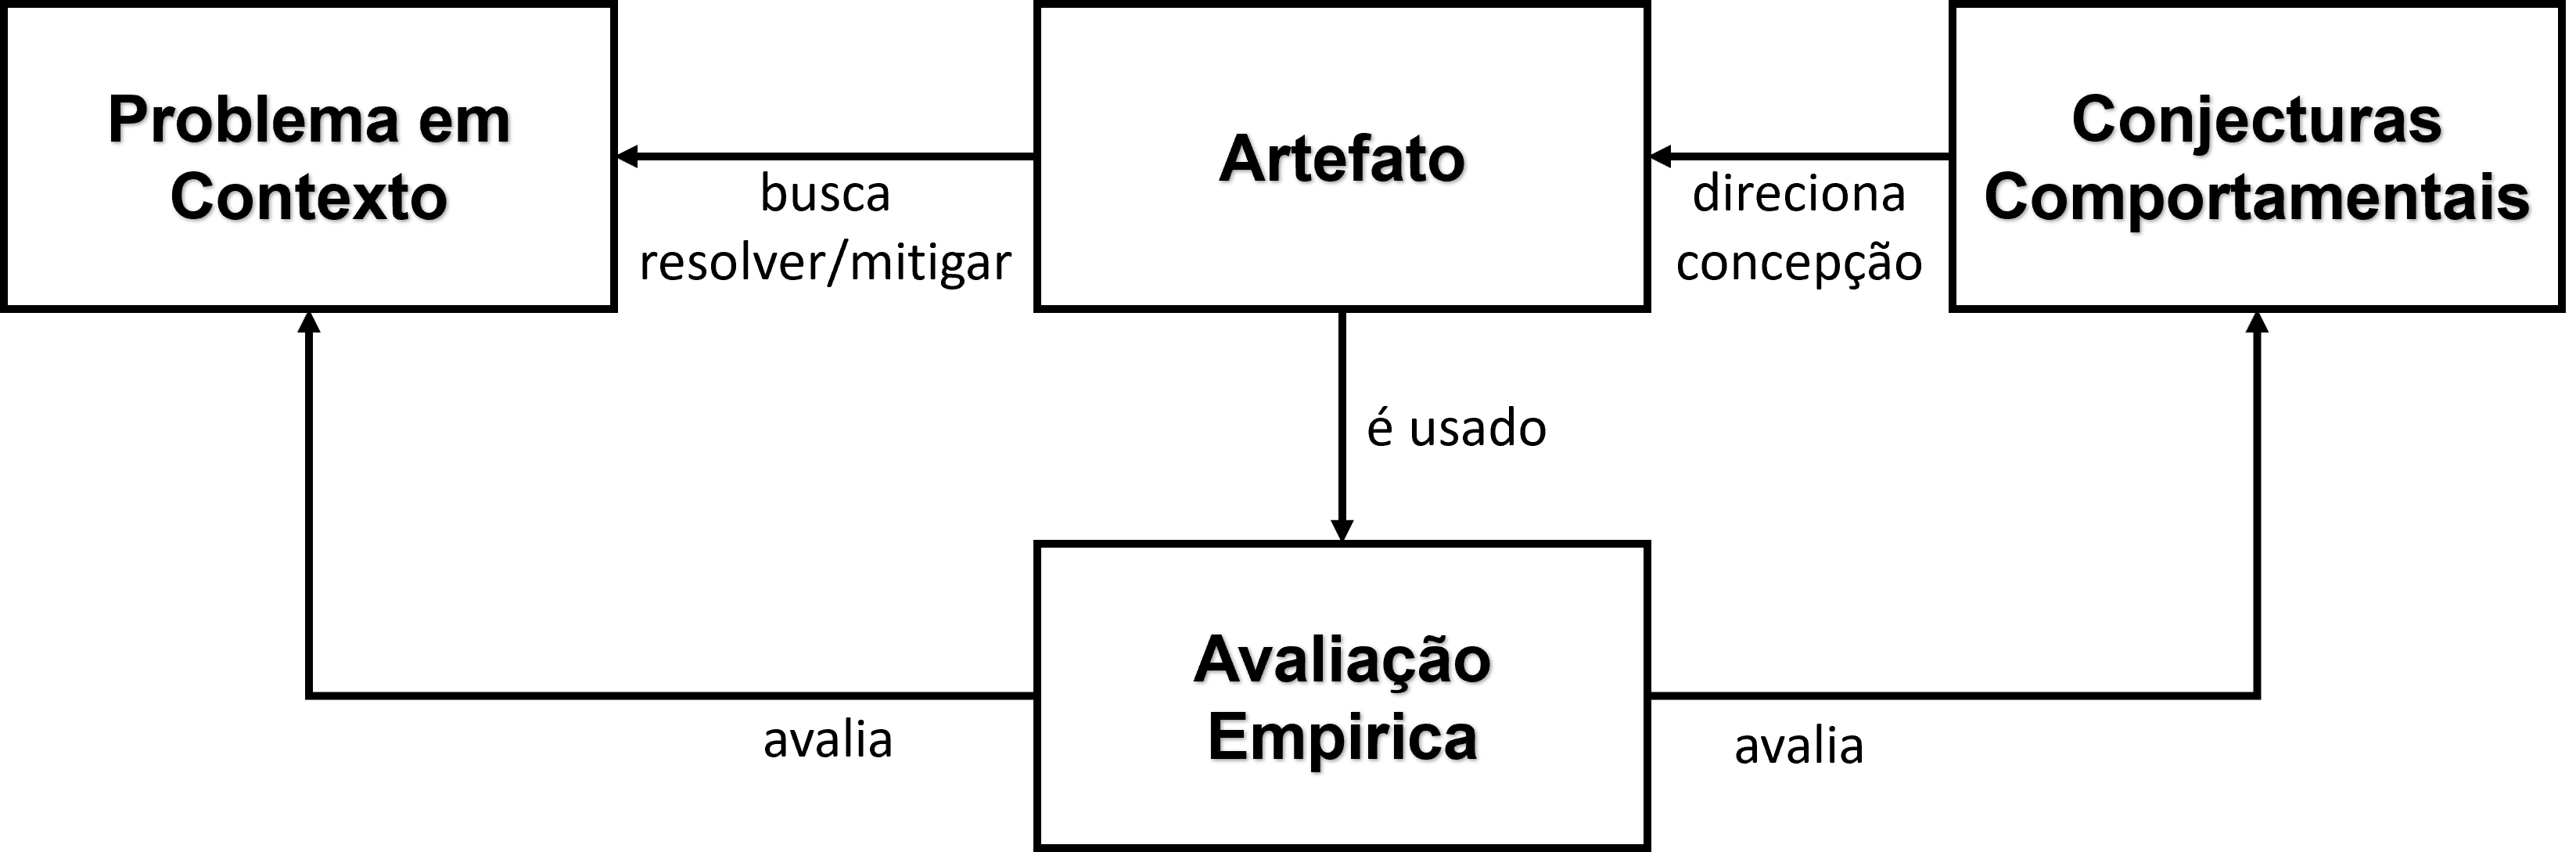
\includegraphics[width=0.5\linewidth]{Images/dsr pimental.png}
    \caption{Elementos centrais do Model-DSR. Baseado em \citep{pimentel2023}}
    \label{fig:dsrmodel}
\end{figure}

O modelo também propõe um diagrama que explicita de forma resumida as conexões entre teoria, problema, solução e contexto. Esse diagrama, junto com sua explicação no formato de texto, é adotado em vários trabalhos do meu grupo para definir a pesquisa que está sendo feita. Exemplos foram dados por \citet{pimentel2019dsr} e \citet{pimentel2023}.

Ao destacar a produção de conhecimento científico como elemento central da DSR, o MODEL-DSR contribui para diferenciar claramente pesquisa de desenvolvimento tecnológico. Ele é especialmente adequado a pesquisas aplicadas em educação mediada por tecnologia, promovendo o rigor metodológico e a relevância prática.

\subsection{Framework de Pesquisa em Tecnologia da Informação}

\citet{march1995design} propuseram um framework bidimensional (ver \autoref{tab:marchsmith}) para pesquisas em Tecnologia da Informação que distingue entre tipos de artefatos produzidos e atividades de pesquisa realizadas. Os artefatos incluem:
\begin{itemize}
    \item \textbf{Construtos}: são os conceitos que formam a linguagem da área de estudo, usados para descrever problemas e formular soluções.
    \item \textbf{Modelos}: expressam relações entre construtos e servem como representacões de situações-problema ou de soluções.
    \item \textbf{Métodos}: são sequências de passos ou algoritmos utilizados para resolver tarefas específicas.
    \item \textbf{Instâncias}: são realizações concretas de sistemas, ferramentas ou protótipos que demonstram o uso prático dos construtos, modelos e métodos.
\end{itemize}

As atividades de pesquisa compreendem:
\begin{itemize}
    \item \textbf{Construção (build)}: desenvolvimento dos artefatos para um objetivo específico, demonstrando sua viabilidade.
    \item \textbf{Avaliação (evaluate)}: análise sistemática do desempenho dos artefatos em função de métricas e critérios estabelecidos.
    \item \textbf{Teorização (theorize)}: construção de explicações que descrevem como e por que os artefatos funcionam em seu ambiente.
    \item \textbf{Justificativa (justify)}: verificação empírica ou formal das teorias propostas, com base em evidências.
\end{itemize}

Esse framework contribui para organizar e avaliar as pesquisas em TI segundo seu tipo de contribuição, facilitando a compreensão e a comunicação dos resultados científicos.

\begin{table}[hbt]
    \centering
    \begin{tabular}{|c|c|c|c|c|}
    \hline
       & Construção & Avaliação & Teorização & Justificativa  \\    \hline
    Construtos &&&&\\     \hline
    Modelo &&&&\\    \hline
    Método &&&&\\    \hline
    Instâncias &&&&\\    \hline
    \end{tabular}
    \caption{O \textit{Framework} de pesquisa em tecnologia da informação proposto por \citet{march1995design}}
    \label{tab:marchsmith}
\end{table}

Além disso,  \citet{hevner2004design} destacam que a contribuição para o corpo de conhecimento científico é um critério essencial para a validade de uma pesquisa baseada em DSR.

\subsection{Como Não Usar  DSR}

A DSR não é uma solução mágica, principalmente não é uma resposta para ser dada no final de uma tese feita por tentativa e erro. 

O principal problema metodológico é o \textit{retrofit}. O candidato, que foi tateando em busca de uma solução para um problema que o agradava, e acabou por esquecer a metodologia, acaba tentando explicar o que fez com uma DSR ``mais ou menos''.

Claro que há uma culpa do orientador, porém quero lembrar que não só o único responsável pela tese é o orientado, como ele é o único que sofre consequências graves pelo seu erro.




\section{A Revisão Bibliográfica}


São dois os objetivos da revisão bibliográfica:
\begin{itemize}
    \item primeiro, ela deve comprovar que o futuro mestre cumpriu bem as fases iniciais da metodologia científica, isso é, o descobrimento e a descrição do problema e a busca de conhecimentos ou instrumentos relevantes ao problema;
    \item realizado isso, ela deve contextualizar o leitor no domínio do conhecimento. 
\end{itemize}

Uma dissertação de mestrado, porém, não é um documento fechado, que tudo explica, mas sim uma revisão dos conceitos do problema e da solução, e um guia para leituras mais detalhadas. 
Elas são similares a artigos de \textit{survey} e deviam, na prática, ser dignas de publicação como tal.

Seus leitores são de dois tipos principais: a banca, que tem alta especialização, e outros pesquisadores que podem buscar a dissertação como referência e modelo de como fazer o trabalho.

A revisão bibliográfica deve ser focada e deve tentar evitar discutir profundamente assuntos não diretamente correlacionados a dissertação.
É importante que a revisão sirva como um guia de leitura dos assuntos, comentado e fazendo ponderações em relação aos documentos citadas.

É costume separar a divisão, possivelmente em dois capítulos, entre a revisão do problema e a revisão das técnicas usadas na dissertação. A abordagem, em geral, é \textit{top-down}, fazendo uma descrição do mais geral ao mais específico.

Na prática, ela não deve ser uma lista de quem disse o quê, mas uma \textbf{revisão global e comparativa do conhecimento}, inclusive com uma visão histórica, e das relações entre aos problemas e propostas analisados.

Nas dissertações onde se resolve um problema específico, esse problema deve ser bem analisado e explicado, e, possivelmente, bem definido, caso não seja definido de forma apropriada na literatura, atendendo ao passo 2 do método científico. 

Finalmente, uma dos objetivos importantes da revisão bibliográfica é fazer uma análise da contribuição de cada texto revisto, de modo a poder contextualizar a contribuição apresentada na dissertação.


\subsection{Revisões Sistemáticas}

Revisões sistemáticas são ferramentas essenciais para a identificação de lacunas no conhecimento e para fundamentar a construção de artefatos na DSR.  \citet{kitchenham2004procedures} definem revisões sistemáticas como um processo rigoroso, transparente e reprodutível de seleção e análise de literatura.

Existem vários modelos similares com estruturas semelhantes que podem ser usados, mas são mais rápidos, como revisões de escopo e revisões rápidas.

A integração de revisões sistemáticas, ou similares, à DSR assegura que a pesquisa se apoie em uma base sólida de conhecimento existente, aumentando sua relevância e contribuição científica.

Para escolher uma forma de revisão, o artigo de \citet{grant2009typology} lista 14 tipos. A partir daí é necessário buscar a descrição da forma mais adequada de fazê-lo. A Linha de Engenharia de Software trabalha há algum tempo com revisões sistematizadas e é possível encontrar não só definições de como devem ser feitas, mas também bons exemplos entre as teses, dissertações e relatórios técnicos do PESC~\footnote{\expurl{https://cos.ufrj.br/index.php/pt-BR/publicacoes-pesquisa}{Publicações do PESC}}

\section{Leituras Adicionais}


O mercado está cheio de livros sobre ``Como fazer uma tese'' e ``Metodologia Científica'' que pouco ajudam. Muitos são voltados para a burocracia da escrita, ensinando quantos centímetros deve ter uma ficha e o formato de uma bibliografia. O problema é bem maior.

Para a área de STEM, esqueça o famoso livro de Umberto Eco, ``Como Fazer uma Tese'', ele é antigo, não é bom para teses de mestrado e doutorado, fala sobre uma ``tesi di laurea'', que é equivalente a um projeto final no Brasil. O livro tem muitos comentários que não se aplicam à engenharia, outras áreas técnicas, e ao Brasil. 

Entre os bons livros que encontrei, estão:
\begin{itemize}
    \item \citet{freitas2001} apresenta um livro prático, de certa forma com uma abordagem similar a este texto, em seu livro \citetitle{freitas2001}. É uma leitura fácil e bastante útil.
\item \citet{woodwell2014} em seu livro \citetitle{woodwell2014} apresenta uma boa introdução à pesquisa e a busca da causalidade, principalmente ligada ao pós-positivismo.
\item \citet{creswell2021projeto} apresentam em \citetitle{creswell2021projeto} uma boa introdução a métodos qualitativos, quantitativos e mistos dentro de vários paradigmas.
\item \citet{Wazla2021} apresenta uma abordagem sobre a metodologia voltada para Computação em seu livro \citetitle{Wazla2021}.
\end{itemize}

Existem outros bons livros no mercado e, possivelmente, seu orientador pode indicar algum.

Se você está interessado em entender melhor como funciona a Ciência, existe uma ampla literatura. 
Para uma visão introdutória e sistemática, recomenda-se a leitura de \citet{chalmers1999o} em sua obra \citetitle{chalmers1999o}, que apresenta e discute o método científico de maneira acessível. 

Um livro  de leitura mais díficil, é \citetitle{Popper1972} de \citet{Popper1972}. 
Já para uma crítica radical à ideia de método fixo na ciência, \citet{feyerabend1975contra} argumenta em \citetitle{feyerabend1975contra} que a ciência avança por vias muitas vezes anárquicas. 
Em outra linha, mas igualmente influente, \citet{kuhn1962estrutura} propõe em \citetitle{kuhn1962estrutura} a noção de paradigmas e revoluções científicas, destacando a descontinuidade no desenvolvimento do conhecimento. Esses três livros compõe uma biblioteca básica e clássica sobre o assunto.

Se a crítica sociológica à ciência te interessa, \citet{collins1993golem} desconstroem o ideal de objetividade científica em \citetitle{collins1993golem}, mostrando como práticas cotidianas e falhas estão presentes até nos experimentos mais renomados, principalmente por meio de estudos de caso. 
De maneira ainda mais provocativa, \citet{latour1987science} examina em \citetitle{latour1987science} como o conhecimento científico é realmente produzido, destacando as redes de atores, laboratórios, disputas e negociações que tornam uma ideia aceita como ``fato''. Ao invés de tratar a ciência como um corpo fixo de verdades, a obra propõe acompanhar a ciência ``em ação'', antes que seus resultados sejam estabilizados. Essa abordagem inaugura os chamados Science and Technology Studies (STS), rompendo com a imagem idealizada de método científico. 
Na mesma direção crítica, \citet{davis1990sonho} refletem sobre os limites da matematização do mundo e a influência do racionalismo cartesiano em \citetitle{davis1990sonho}, questionando se a matemática é descoberta ou invenção, e como ela molda — ou distorce — nossa compreensão da realidade.